\section{Synchronisation in verteilen Systemen}
\label{cap:Uhrenarten}
\subsection{Systemmodell}
% Events: senden, empfangen, internal
Dieser Abschnitt beschreibt ein vereinfachtes Modell eines verteilten Systems, welches als Grundlage für alle weiteren Ausführungen heran gezogen wird.
Zur Vereinfachung wird ein sehr grundlegendes Modell verwendet, welches jedoch ausreichend ist um die in dieser Arbeit geschilderten Zusammenhänge korrekt und ohne Beschränkung der Allgemeinheit darzustellen.

In unserem Modell besteht ein verteiltes System aus $n$ Prozesse die durch die Menge $P=\{p_1, p_2,\ldots, p_n\}$ beschrieben sind.
Die Prozesse können lediglich durch das Senden und Empfangen von Nachrichten kommunizieren.
Dabei wird angenommen, dass Nachrichten zuverlässig verschickt werden und somit in jedem Fall, nach einer gewissen endlichen Verzögerung, beim Empfänger ankommen.
Nachrichten müssen nicht zwangsläufig in der selben Reihenfolge ankommen in der sie gesendet wurden.
Dies ist dem Übertragungsweg geschuldet.

Ein Prozess $p_i$ besteht aus einer Sequenz von Ereignissen $E_i=\{e_i^1, e_i^2, \ldots\}$, welche eine totale Ordnung aufweist.
Diese Ordnung ergibt sich durch den Programmablauf des Prozesses und wird durch die Relation $\rightarrow$ beschrieben.
Löst ein Prozess $p_i$ zum Beispiel zuerst ein Ereignis $e_i^x$ aus und anschließend ein Zweites $e_i^y$, gilt $e_i^x \rightarrow e_i^y$. 
Die Menge $E$ enthält alle Ereignisse die im gesamten System auftreten.
\fig{fig:genericEvents} zeigt eine exemplarische Kommunikation zwischen drei Prozessen und deren Ereignisse.
Dabei werden nur Sende- und Empfangsereignisse betrachtet.

Jedes Ereignis ist atomar und stellt eine Zustandsänderung des dazugehörigen Prozesses dar.
Für die in dieser Arbeit beschriebenen Verfahren sind von besonderer Interesse die \qq{gesendet}- und \qq{empfangen}-Ereignisse.
Diese Ereignisse weisen Abhängigkeiten unter den Prozessen auf, welche die Notwendigkeit schafft die Prozesskommunikation zu synchronisieren.
Beiden Ereignisse können daher als Erweiterung der lokalen Programmordnung eines Prozesses auf das verteilte System betrachtet werden.

\begin{figure}[ht]
    \centering
    \includegraphics[width=10cm]{2_generic_events.pdf}
    \caption[Beispiel einer beliebigen Kommunikation]{Darstellung einer auf Nachrichten basierten Kommunikation dreier Prozesse. Ereignisse sind als schwarze Punkte auf den Zeitstrahlen und Nachrichten als Pfeile dargestellt.}
    \label{fig:genericEvents}
\end{figure}

Außerdem geht unser Modell davon aus, dass ein Prozess aus drei Schichten besteht.
Dies ist für die theoretische Definition unwesentlich, erleichtert aber die praktische Umsetzung und verbessert das Verständnis.
Die höchste Schicht ist die Anwendungsschicht, hier wird die Applikationslogik implementiert die durch das verteilte System abgebildet werden soll.
In der mittleren Schicht wird die Synchronisation der Kommunikation vorgenommen und kann somit für die Anwendungsschicht transparent  erfolgen.
Die unterste Schicht stellt die Netzwerkschicht dar, die Aufgabe dieser Schicht ist es die Nachrichten physikalisch zu übertragen.

\subsection{Kausalität und Ordnung}
\label{cap:ordnung}
% ungeordnet
% kausale Ordnung
% partielle kausale Ordnung
% totale Ordnung
Die meisten Menschen würden sicherlich dem zustimmen, dass ein Ereignis $a$ vor einem Ereignis $b$ passierte, wenn $a$ zu einem früheren Zeitpunkt als $b$ auftrat.
Das Konzept \qq{Zeit} ist fundamental in unserer Art zu denken verankert.
Es ist von dem grundlegenderen Konzept der Ordnung in der Ereignisse eintreten abgeleitet.
Die zeitliche Ordnung von Ereignissen bestimmt die Art wie wir über die Funktionsweise von Systeme denken \cite{Lamport1978}.

Dies führt zu Überlegungen über den Zusammenhang von Ursache und Wirkung.
Die Verbindung zwischen dem auslösenden Ereignis und dem ausgelösten Ereignis wird als Kausalität bezeichnet.
Es wird also die Abfolge von aufeinander bezogenen Ereignisse oder Zustände betrachtet.
Meist ist es nicht direkt ersichtlich ob Ereignisse kausal zusammenhängen, hierzu müssen die Gegebenheiten und Zusammenhänge der Ereignisse genau bekannt sein.
Dies ist nicht immer gegeben und auch nicht einfach entscheidbar, da hierzu Zusammenhänge betrachtet werden müssen, die meist in einer höhreren Schicht gegeben sind oder schlichtweg für einen Computer nicht erfassbar sind.
Daher wird im folgenden immer von potentieller Kausalität gesprochen.
Das bedeutet, dass nur Aussagen darüber gemacht werden ob ein Ereignis die Ursache für ein Anderes sein kann.

In einem einzelnen nicht nebenläufigen Prozess ist die Kausalität durch den Programmablauf gegeben.
Da die Instruktionen eines Programmes nacheinander ohne Vergabelungen ausgeführt werden und dabei jede Instruktion atomar ist, kann der aktuelle Zustand nur aus den davor ausgeführten Instruktionen bestimmt worden sein.
Hierbei kann eine Instruktion analog zu einem Ereignis verstanden werden.

Im Vergleich hierzu ist die Situation in einem verteilten System oder nebenläufigen Prozess deutlich komplexer.
Durch die Verteilung und Parallelität des Programmcodes ist die \qq{natürliche} Ordnung nicht mehr gegeben.
Innerhalb eines Prozesses ist die Ordnung weiterhin gegeben, da sich ein lokaler Prozess wie oben geschildert verhält.
Wird nun aber das Gesamtbild, also das ganze System betrachtet, sind die obigen Eigenschaften nicht mehr gegeben.
Das Wissen um die Kausalität der Ereignisse ist jedoch häufig notwendig um die Konsistenz des Systems zu wahren.

Der potentielle kausale Zusammenhang zwischen Ereignisse kann durch die Zeit festgestellt werden.
Ein Ereignis, welches zu einem späteren Zeitpunkt eingetreten ist, kann unmöglich die Ursache für ein vorhergehendes Ereignis sein.
Sind also die Zeitpunkte der Ereignisse bekannt, kann eine Aussage über die Kausalität getroffen werden.
Menschen haben ein intuitives Verständnis solcher Zusammenhänge.

Eine zeitliche Ordnung der Ereignisse ist somit die Grundlage für die Erkennung kausaler Zusammenhänge.
Ein Computer hat natürlich kein intuitives Verständnis von Zeit.
Daher müssen einige mathematische Definitionen festgelegt werden, welche die Grundlage für die Implementierung der zeitlichen Ordnungen dienen.

Damit eine Ordnung hergestellt werden kann, müssen die Ereignisse in Relation gesetzt werden können.
Eine Relation wurde bereits beschrieben, nämlich die \textit{Programmablaufrelation} $\rightarrow$.
Lamport \cite{Lamport1978} definiert in seiner Arbeit die \textit{happend before} Relation $\Rightarrow$ und stellt die kleinste Relation dar, die folgende Bedingungen erfüllt:
\begin{itemize}
    \item Wenn $e_i^x \rightarrow e_i^y$, dann $e_i^x \Rightarrow e_i^y$.
    \item Wenn $e_i^x$ ein Sendeereignis ist und $e_j^y$ das Empfangsereignis der selben Nachricht darstellt, dann folgt $e_i^x \Rightarrow e_j^y$.
    \item Wenn $e_i^x \Rightarrow e_j^y$ und $e_j^y \Rightarrow e_k^z$, dann $e_i^x \Rightarrow e_k^z$.
\end{itemize}

Aus der ersten Bedingung ist ersichtlich, dass aus der strengeren Programmordnung direkt die happend before Relation für zwei lokale Ereignisse abgeleitet werden kann.
Die zweite Bedingung fordert, dass das Empfangsereignis einer Nachricht nie vor dem entsprechenden Sendeereignis eintreten kann.
Offensichtlich kann also eine Nachricht nicht empfangen werden, wenn sie noch nicht verschickt wurde.
Dieser Zusammenhang ist für Menschen zwar intuitiv ersichtlich kann nun aber auch für Computer korrekt formuliert werden.
Durch die dritte Bedingung ist die Transitivität der Relation gegeben.
Wurde ein Ereignis $z$ nach $y$ ausgelöst und $x$ vor $y$ gilt logischerweise, dass $x$ auch vor $z$ ausgelöst werden musste und somit $x\Rightarrow z$ gilt.

Ein Ereignis $e_j^y$ gilt als kausal abhängig von $e_i^x$ wenn $e_i^x \Rightarrow e_j^y$, da es nur ausgeführt werden kann wenn die Ausführung von $e_i^x$ bereits abgeschlossen ist.
Alternativ kann $e_i^x$ als Vorbedingung von $e_j^y$ betrachtet werden.
In dieser Notation gibt das Subskript den Index des Prozesses an und das Superskript die Postions des Ereignisses für den lokalen Prozess.

Zwei Ereignisse gelten als gleichzeitig aufgetreten wenn $e_i^x \centernot\Rightarrow e_j^y$ und $e_j^y \centernot\Rightarrow e_i^x$ gilt.
Dann können beide Ereignisse parallel ausgeführt werden, da sie sich nicht gegenseitig kausal beeinflussen können.
Diese Nebenläufigkeit wird in Symbolen als $e_i^x \parallel e_j^y$ geschrieben.

Es ist offensichtlich, dass jede korrekte logische Uhr die happend before Relation einhalten muss.
Lamport folgert daraus die Uhrenbedingung (engl. \qq{clock condition}), die von jeder korrekten logischen Uhr erfüllt werden muss \cite{Lamport1978}:
\begin{equation*}
\forall e_i^x, e_j^y \in E \colon \text{wenn } e_i^x \Rightarrow e_j^y \text{ dann } C(e_i^x) < C(e_j^y)
\end{equation*}

In Worte gefasst bedeutet diese Bedingung, dass die Uhren zweier Ereignisse durch die \textit{kleiner als} Relation die kausale happend before Relation bestimmen.
Der Größenvergleich der Uhren gibt also Aufschluss über die kausale Abhängigkeit der Ereignisse.
Aus dieser Uhrenbedingung lassen sich zwei konkrete Bedingungen ableiten, welche sich direkt aus der Definition der $\Rightarrow$ Relation ergeben:
\begin{itemize}
    \item Wenn $e_i^x \rightarrow e_i^y$, dann $C(e_i^x) < C(e_i^y)$.
    \item Wenn $e_i^x$ ein Sendeereignis ist und $e_j^y$ das Empfangsereignis der selben Nachricht darstellt, dann folgt $C(e_i^x) < C(e_i^y)$.
\end{itemize}

Die dritte Bedingung aus der Definition der happend before Relation muss hier nicht explizit wiederholt werden, da diese lediglich die Transitivität beschreibt und diese durch die $<$ Relation der Uhren gegeben ist.

Die eingeführten Regeln erlauben es nun die Zusammenhänge zwischen Ereignisse genauer zu betrachten.
Zustellungsregeln (engl. \qq{delivery rules}) definieren Einschränkungen an der Reihenfolge wie eingehende Nachrichten an den zu verarbeiteten Prozess verschickt werden dürfen.
Eine wichtige Regel ist die FIFO-Zustellung (engl. \qq{first in first out delivery}) die besagt, dass ein Prozess $j$ Nachrichten in der selben Reihenfolge empfangen muss wie sie von $i$ versendet wurden.
Dabei können Nachrichten von anderen Prozessen in beliebiger Reihenfolge versandt werden.
Es gilt somit
\begin{equation*}
    \text{wenn } e_i^s \rightarrow e_i^S \text{ dann } e_j^r \rightarrow e_j^R,
\end{equation*}
wobei $s$ und $S$ Sendeereignisse darstellen und $r/R$ die entsprechenden Empfangsereignisse sind.
In dieser Definition ist keine bestimmte Reihenfolge an Ereignisse von anderen Prozessen gefordert.

Eine weitere, im Vergleich zur FIFO-Zustellung strengere, Zustellungsregel ist die kausale Zustellung (engl. \qq{causal delivery}). Diese ist gegeben 
\begin{equation*}
    \text{wenn } e_i^s \Rightarrow e_k^S \text{ dann } e_j^r \rightarrow e_j^R.
\end{equation*}

Kausale Zustellung erweitert die FIFO-Zustellung um die Einschränkung, dass gesendete Nachrichten von verschiedenen Prozessen geordnet werden, sofern diese kausal nach der happend before Relation zusammenhängen.

Damit ein kausale Zustellung implementiert werden kann, muss die Uhr in der Lage sein Aussetzer in der Kommunikation zu erkennen.
Diese Eigenschaft wird \textit{gap detection} genannt.
Sie beschreibt den Umstand, dass ein Prozess in der Lage sein muss anhand zweier eingehender Nachrichten und deren Zeitstempel erkennen können muss, dass eine Nachricht existiert die in der Reihenfolge zwischen den beiden vorhanden Nachrichten gehört und bisher nicht empfangen wurde.
Formell gesprochen muss für zwei gegebenen Uhren $C_i(e_i^x) < C_j(e_j^y)$ entschieden werden, ob ein Ereignis $e_k^z$ mit $C_i(e_i^x)<C_k(e_k^z)<C_j(e_j^y)$ existiert \cite{babaoglu1993consistent}.

\subsection{Uhren}
In diesem Kapitel werden unterschiedliche Uhrtypen vorgestellt.
Generell wird zwischen physikalischen und logischen Uhren unterschieden \cite{Tanenbaum2007}.
Die im vorherigen Abschnitt beschrieben Zusammenhänge ermöglichen es logische Uhren formell zu definieren.
Bevor jedoch logische Uhren genauer beschrieben werden, wird zu erst auf physikalische Uhren eingegangen um den Unterschied zu logischen Uhren und deren Motivation zu verdeutlichen.

\subsubsection{Physikalische Uhren}
In der Regel besitzen heutige CPUs Schaltkreise die als Zeitgeber für die Uhrzeit verwendet werden.
Obwohl häufig als Uhr bezeichnet handelt es sich hierbei viel mehr um einen Zähler.
Ein im Prozessor integrierter Quarzkristall schwingt bei angelegter Spannung mit einer fest definierten Frequenz.
Mit dieser gegeben Frequenz kann nun ein Zähler pro Sekunde einmal inkrementiert werden und somit als Zeitgeber verwendet werden.

Bisher wurde die Darstellung eines Zeitpunktes weitestgehend ignoriert. Es liegt nahe, dass die für Menschen intuitive aufgeteilte Darstellung von Datum und Uhrzeit für Computer umständlich ist. Daher gibt es unterschiedliche Systeme, wie ein Zeitpunkt dargestellt werden kann.

Ein gängiges System um Zeitpunkte zu bestimmen ist die Unixzeit.
Dabei werden alle Sekunden seit dem 1. Januar 1970 um 00:00:00 Uhr UTC gezählt.
Ein Zeitpunkt kann daher einfach als Ganzzahl dargestellt werden.
Der große Vorteil dieses Systems liegt in seiner Einfachheit.
So kann mit einer Rechenoperation die Zeitdauer zwischen zwei Timestampes berechnen oder durch einen einfachen Vergleich festgestellt werden, welcher Timestamp weiter in der Vergangenheit liegt.

Wird nun jedem Ereignis in einem verteilten System ein Unix-Timestamp zugewiesen, kann theoretisch eine zeitliche Ordnung der Ereignisse über Prozessgrenze hinaus erreicht werden. Dies wird durch eine einfache Sortierung nach dem Zeitstempel erzielt.
Ein Problem dieser Herangehensweise ist die Auflösung des Zeitstempels. Treten mehrere Ereignisse innerhalb einer Sekunde auf, kann ihre Reihenfolge nicht am Timestamp festgestellt werden, da sich dieser logischerweise nur jede Sekunde ändert.

Hier ist die Unixzeit nicht mehr ausreichend und eine genauere Darstellung muss gewählt werden.
Dabei steigt jedoch die Komplexität bei der Verarbeitung der Zeitstempel.
Zusätzlich ist nicht sofort klar, welche Darstellung als genau genug gilt.
Je kleiner der zeitliche Unterschied zwischen zwei Zeitstempeln desto genauer das System.
Hierbei muss ein Kompromiss zwischen Genauigkeit, Speicherbedarf und Verarbeitungsaufwand gefunden werden.

Ein weiteres Problem von physikalischen Uhren ist ihre Abweichung von der tatsächlichen Zeit.
So besitzt jeder Quartzkristall eine gewisse Schwankung in seiner Frequenz.
Dadurch driftet die Computeruhr immer weiter von der tatsächlichen Zeit ab \cite{Coulouris2011}[S. 598].
Umgangssprachlich würde man sagen, die Uhr geht vor bzw. nach.
Dieses Abdriften lässt sich nur durch Verwendung von genaueren Uhren wie z.B. Atomuhren vermeiden.
Es ist jedoch unpraktikabel in jeden Computer eine Atomuhr zu installieren, daher muss die Uhr eines Computers mit einer anderen exakten Uhr regelmäßig synchronisiert werden.
In Netzwerken wird hierzu in der Regel das, in der Einleitung erwähnte, Network Time Protocol verwendet \cite{Coulouris2011}[S. 603].

Eine für verteilte Systeme besser geeigneter Algorithmus zum korrigieren der Uhrabweichungen stellt der Berkeley-Algorithmus \cite{gusella1989accuracy} dar.
Dieser erfordert jedoch einen globalen Zeitgeber, der im Gegensatz zu NTP, aktiv die Zeit im System verteilt.

Im Allgemeinen wird in verteilten Systemen davon ausgegangen, dass keine globale Uhr existiert und somit physikalische Uhren nicht zur Anwendung kommen \cite{Tanenbaum2007}[S. 11].
Für ein verteiltes System kann der absolute Fehler einer Uhr vernachlässigt werden, solang alle beteiligten Prozesse den selben Fehler haben und somit relativ innerhalb des Systems richtig sind.
Liegen zum Beispiel die Uhren aller Prozesse exakt 10 Sekunden in der Vergangenheit, kann die Reihenfolge der Ereignisse immer noch festgestellt werden. 
Weisen jedoch nur manche Prozesse einen Fehler auf, kann die Reihenfolge nicht mehr korrekt aus den Zeitstempel erschlossen werden.
Ist die Zeit aller Prozesse systemintern konsistent, kann auf eine Synchronisation einer externen realen Zeit verzichtet werden \cite{bengel2015masterkurs}[S. 359].
Diese Überlegung führt zu der Definition von logischen Uhren.

\subsubsection{Lamport-Uhren}
\label{cap:vectorclock}
Leslie Lamport beschreibt in seinem Paper \cite{Lamport1978}, indem er gleichzeitig kausale Ordnung definiert, ein Verfahren um Prozesse durch logische Uhren zu synchronisieren.
Sein vorgeschlagener Algorithmus ist heute als Lamport-Uhr bekannt und stellt eine simple Möglichkeit dar, partielle Ordnung in einem verteilen System herzustellen.

Lamport führt den Begriff der logischen Zeit ein.
Hierbei verläuft die logische Zeit diskret und schreitet nur voran, wenn ein Ereignis eintritt \cite{leon2013ereignisdiskrete}[S. 462].
Eine logische Uhr erfasst die logische Zeit indem bei Eintritt eines Ereignisses ein Zähler inkrementiert wird.
Dabei hält jeder Prozess einen eigenen Zähler.
Sendet nun ein Prozess eine Nachricht, hängt er seinen aktuellen Zählerstand als Zeitstempel an die Nachricht an.
Empfängt nun ein anderer Prozess eine Nachricht kann er anhand des Zeitstempels der Nachricht und seiner lokalen Uhr den kausalen Zusammenhang erschließen.

Formal ist eine Lamport-Uhr $C$, wie alle logische Uhren, als eine Funktion definiert, welche einem Ereignis $e$ eine Nummer $C(e)$ zuweist.
Lamport-Uhren erfüllen die Uhrbedinung aus Abschnitt~\ref{cap:ordnung}, indem jeder Prozess $i$ seine eigene Uhr $C_i$ hält und nach folgenden Regel aktualisiert \cite{Lamport1978}:
\begin{itemize}
    \item Wenn $e_i^x$ kein Empfangsereignis ist, dann $C_i(e_i^x):=C_i(e_i^{x-1})+1$
    \item Ist $e_i^x$ ein Empfang-Ereignis der Nachricht $m$, dann $C_i(e_i^x):=\max\{C_i(e_i^{x-1}), C_j(e_j^y)  \} + 1$, wobei Prozess $j$ die Nachricht $m$ an $i$ geschickt hat und $C_j(e_j^y)$ der Uhrwert des Sende-Ereignis ist.
\end{itemize}

\fig{fig:lamportBsp} zeigt eine exemplarische Kommunikation zwischen drei Prozessen, dabei wird die Lamport-Uhr zum Zeitpunkt eines Ereignisses als Zahl in der Grafik dargestellt.
Lamport bewies, dass seine Uhr die Uhrenbedingung erfüllt \cite{Lamport1978}.
Hierbei muss gezeigt werden, dass die aus der Uhrbedingung abgeleiteten Bedingungen erfüllt sind.
Wird eine Nachricht versendet, muss die lokale Lamport-Uhr inkrementiert werden. 
Daraus folgt, dass für zwei direkt aufeinander folgenden Sende-Ereignisse $e_i^x$ und $e_i^y$ wobei $e_i^x \rightarrow e_i^y$ gilt $C(e_i^x) < C(e_i^y)$, da bei Eintritt von $e_i^x$ die Uhr auf $a$ inkrementiert wurde und bei $e_i^y$ auf $a + 1$ erhöht werden musste.

\begin{figure}[ht]
    \centering
    \includegraphics[width=10cm]{LamportBeispiel.pdf}
    \caption[Exemplarische Kommunikation mit Lamport-Uhr]{Kommunikation zwischen drei Prozessen unter Verwendung von Lamport-Uhren.}
    Nachgezeichnet aus  \cite{landes2006dynamic}
    \label{fig:lamportBsp}
\end{figure}

Die zweite Bedingung fordert, dass für ein Sendeereignis $e_i^x$ die Uhr einen kleineren Wert als die des entsprechenden Empfangsereignis $e_j^y$ besitzt.
Durch die $\max$-Funktion wird zwischen der lokalen Uhr und der an die Nachricht angehängte Uhr entschieden.
Hieraus entstehen zwei Fälle:
Im ersten Fall ist der Zähler der lokalen Uhr größer als die der Nachricht.
Somit ist die Nachricht älter als der aktuelle lokale Zustand und die lokale Uhr inkrementiert um Eins stellt den neuen Uhrenwert dar.
Im zweiten Fall ist die Uhr der Nachricht größer als die lokale Uhr.
Dem Empfänger sind also nicht alle Ereignisse des Sendeprozesses bekannt und hat somit einen älteren Stand.
In diesem Fall wird die Uhr aus der Nachricht als neue Uhr übernommen und inkrementiert.
In beiden Fällen gibt die Uhr für das Sendeereignis immer einen kleineren Wert als für das Empfangsereignis an somit ist $C(e_i^x) < C(e_j^y)$ erfüllt.

Lamport-Uhren haben jedoch einen entscheidenden Nachteil.
Mit ihnen können keine Unterbrechungen erkannt werden.
Da dies jedoch die Grundlage für kausaler und FIFO-Zustellung ist, sind Lamport-Uhren nicht dafür geeignet diese zu garantieren.
Der Grund hierfür ist, dass keine Information über den Zustand der anderen Prozesse gespeichert wird \cite{landes2006dynamic}.

Haben zwei Ereignisse den selben Zählerstand müssen diese gleichzeitig aufgetreten sein.
Ist also $C_i(e_i^x)=C_j(e_j^y)$ gegeben, folgt $e_i^x \parallel e_j^y$.
Gilt jedoch $C_i(e_i^x)<C_j(e_j^y)$ ist es nicht möglich zu entscheiden ob $e_i^x \Rightarrow e_j^y$ oder $e_i^x \parallel e_j^y$ gilt.
Die Uhr erlaubt es also nicht eine Aussage über die Reihenfolge der Ereignisse selbst zu machen \cite{landes2006dynamic}.

Lamport-Uhren sind jedoch dazu geeignet eine totale Ordnung im System herzustellen.
Diese strikte Ordnung muss jedoch mit einer großen Anzahl an verschickten Nachrichten bezahlt werden, was wieder eine hohe Netzwerklast mit sich bringt.
Es würde daher ausreichen, Ereignisse nach ihrem kausalen Zusammenhang zu ordnen.
\fig{fig:LamportConcurrent} zeigt eine solche Situation, in der eine kausale Ordnung ausreichen würde, da das Empfangen von Nachricht $m_2$ nicht davon abhängt ob $m_2$ bereits empfangen wurde.
Eine totale Ordnung würde jedoch dazu führen, dass $m_1$ und $m_2$ von jedem Prozess in der selben Reihenfolge empfangen werden.
Ferner ist es nicht möglich ob das Versenden von $m_3$ vom Empfangen von $m_1$ oder $m_2$ abhängt \cite{Tanenbaum2007}[S. 249].

\begin{figure}[ht]
    \centering
    \includegraphics[width=0.3\textwidth]{LamportConcurrent.png}
    \caption[Lamportuhren und Kausalität]{Nebenläufige Nachrichtenübertragung unter Verwendung von Lamportuhren.}
    Quelle: \cite{Tanenbaum2007}
    \label{fig:LamportConcurrent}
\end{figure}

Mit Lamport-Uhren können Ereignisse somit nach ihren kausalen Abhängigkeiten geordnet werden.
Es kann jedoch keine Aussage über die Abhängigkeiten selbst getroffen werden.
So kann zum Beispiel nicht entschieden werden ob zwei Ereignisse in der kausalen Ordnung vertauscht werden können ohne die kausale Konsistenz zu zerstören.
Hierzu müssen zusätzliche Informationen über die restlichen Prozesse gespeichert werden \cite{landes2006dynamic}.

% negativ Beispiel in Plausible Clocks Constant Size Logical Clocks for Distributed Systems
\subsubsection{Vektoruhren}
Vektoruhren stellen eine Erweiterung der von Lamport vorgestellten Uhr dar und werden häufig eingesetzt um die Defizite der Lamport-Uhr zu beheben.
Statt einem einzelnen skalaren Zeitstempel, verwenden Vektoruhren viele Zähler um die kausale Abhängigkeit zwischen Ereignisse umfänglicher zu erfassen, als dies mit Lamport-Uhren möglich wäre.
Ihr Name wurde ihnen gegeben, da die Zeitstempel in einem Vektor zusammengefasst werden.
Sie wurden zeitgleich von Mattern \cite{mattern1989virtual} und Fidge \cite{fidge1991logical, fidge1988timestamps} vorgeschlagen und analysiert.

Wie bei Lamport-Uhren verwaltet jeder Prozess seine eigne lokale Uhr.
Die Uhr ist jedoch nun ein Vektor aus $n$ skalaren Werten, bei einem System bestehend aus $n$ Prozesse.
Jede Komponente $VC_i(e_i^x)[j]$ entspricht dem letzten Uhrenwert den Prozess $i$ zu Prozess $j$ zum Zeitpunkt $e_i^x$ kennt.
Folgende Regeln müssen bei der Aktualisierung der Uhr eingehalten werden:
\begin{itemize}
    \item Wenn $e_i^x$ das Empfangsereignis der Nachricht $m$ ist, dann $VC_i(e_i^x):=\max\{ VC_i(e_i^{x-1}), VC_j(e_j^y) \}$, wobei $VC_j(e_j^y)$ der Uhrenvektor des Sendeereignisses von Prozess $j$ ist, welcher die Nachricht $m$ an Prozess $i$ gesendet hat. Das Maximum wird komponentenweise bestimmt.
    \item Wenn $e_i^x$ ein beliebiges Ereignis ist, dann muss der Prozess seine Vektorkomponente inkrementiert: $VC_i(e_i^x)[i]:=VC_i(e_i^{x-1})[i] + 1$. Dies beinhaltet auch Empfangsereignisse.
\end{itemize}

\fig{fig:VektorBsp} zeigt den selben Kommunikationsverlauf wie \fig{fig:lamportBsp} jedoch mit der Verwendung von Vektoruhren statt Lamport-Uhren.
Anschaulich betrachtet ist $\VCieix[i]$ gleich der Anzahl der von Prozess $i$ bereits ausgeführten Ereignisse (inklusive $\eix$) zum Zeitpunkt von $\eix$.
Nach der selben Logik gibt $\VCieix[j]$ die Anzahl der Ereignisse von Prozess $i$ an, die vor $\eix$ eingetreten sind.

\begin{figure}[ht]
    \centering
    \includegraphics[width=10cm]{VektorBeispiel.pdf}
    \caption[Exemplarische Kommunikation mit Vektoruhren]{Kommunikation dreier Prozessen unter Verwendung von Vektoruhren.}
    Nachgezeichnet aus  \cite{landes2006dynamic}
    \label{fig:VektorBsp}
\end{figure}

Ein Vorteil von Vektoruhren ist, dass sie nicht nur die schwache Uhrenbedingung erfüllen sondern auch eine strengere Variation, nämlich die starke Uhrenbedingung \cite{Lamport1978}:
\begin{equation*}
\forall e_i^x, e_j^y \in E \colon VC(e_i^x) < VC(e_j^y) \text{ genau dann, wenn } e_i^x \Rightarrow e_j^y
\end{equation*}

Bei Lamport-Uhren, welche nur die schwache Uhrenbedingung erfüllen, ist die Aussage $C_i(e_i^x)<C_j(e_j^y)$ doppeldeutig. 
Es kann nicht zwischen $e_i^x \Rightarrow e_j^y$ oder $e_i^x \parallel e_j^y$ unterschieden werden.
Bei Uhren die jedoch die starke Uhrenbedingung erfüllen, wie Vektoruhren, lässt die selbe Aussage nur den Schluss zu, dass $e_i^x \Rightarrow e_j^y$ gelten muss \cite{leon2013ereignisdiskrete}[S. 465].
Somit wurde die Schwäche der Lamport-Uhr eliminiert.

Damit die starke Uhrenbedingung von Vektoruhren erfüllt werden kann, muss zuerst die $<$~Relation von Vektoruhren definiert werden \cite{mattern1989virtual}:
\begin{align*}
\VCieix &< \VCjejy \text{ genau dann, wenn} \\
       & \VCieix \ne \VCjejy \text{ und } \\
       & \forall k | 1 \leq k \leq n \colon \VCieix[k] \leq \VCjejy[k].
\end{align*}

Nun kann anhand einer Vektoruhr entscheiden werden ob ein Ereignis kausal abhängig von einem Anderen ist:
\begin{equation*}
    \eix \Rightarrow \ejy \text{ genau dann, wenn } \VCieix[i] \leq \VCjejy[i].
\end{equation*}

Hervorzuheben ist, dass nur eine einzige skalare Operation notwendig ist, um diesen Zusammenhang zu erschließen.
Ferner ist die obige Formel nicht symmetrisch.
Wird sie angewendet und ergibt $\eix \centernot\Rightarrow \ejy$, muss sie ein zweites Mal angewendet werden um zwischen $\ejy \Rightarrow \eix$ oder $\eix \parallel \ejy$ zu entscheiden.
Dies führt zu dem Nebenläufigkeitstest \cite{landes2006dynamic}:
\begin{align*}
    \eix \parallel & \ejy \text{ genau dann, wenn } \\
                   & \VCjejy[i] \le \VCieix[i] \text{ und } \\
                   & \VCieix[j] \le \VCjejy[j].
\end{align*}

Ergibt der Test $\eix \centernot\parallel \ejy$ kann direkt anhand des nicht erfüllten Terms der beiden Bedingungen entschieden werden ob $\eix \Rightarrow \ejy$ oder $\ejy \Rightarrow \eix$ gilt.

Der große Nachteil von Vektoruhren besteht darin, dass ein fixer Index verwendet wird, um die Komponenten im Vektor auszuwählen die den skalaren Uhrenwert eines Prozesses darstellt.
Dies führt zu zwei sehr einschränkenden Voraussetzungen.
Zum einen muss die Anzahl der Prozesse konstant und zum anderen auch im Voraus bekannt sein.
In dynamischen System stellen diese beiden Einschränkungen ein ernstes Problem dar, da die Anzahl in solchen System nicht einfach zu bestimmen ist, was in der Natur der Sache liegt \cite{landes2006dynamic}.

\subsubsection{Interval Tree Clocks}
\label{cap:itc}
Vektoruhren haben den großen Nachteil für dynamischen Systeme eher ungeeignet zu sein.
Daher ist es interessant entsprechende neue Verfahren zu untersuchen, welche die Defizite von Vektoruhren in einem solchen Kontext ausmerzen.
Interval Tree Clocks (ITC) stellen ein solches Verfahren dar und wurden 2008 von \etal{Almeida} in ihrer Arbeit \qq{Interval Tree Clocks: A Logical Clock for Dynamic Systems} \cite{almeida2008treeclocks} vorgeschlagen.
Wie bereits angedeutet, sind ITCs besonders für dynamische Systeme geeignet, in denen häufig Prozesse gestartet und terminiert werden.
Während Vektoruhren eine globale ID benötigen, nämlich den Index der Vektorkomponente, kommen ITCs ohne solcher globalen eindeutigen IDs aus. Dies ermöglicht eine gänzlich dezentrale Erzeugung von Prozessen \cite{almeida2008treeclocks}.

Interval Tree Clocks haben eine in der Größe variable Darstellung, welche sich automatisch an der Anzahl der existierenden Prozesse richtet. Die Größe der Uhren nimmt zu und ab, entsprechend der im System aktiven Prozesse.
Um dies zu erreichen setzten ITCs auf dem \qq{Fork-Event-Join}-Modell auf.
Hierbei handelt es sich um ein Modell bei dem die Kausalität durch drei grundlegende Operationen beschrieben werden kann.
Diese Operationen, \textit{fork}, \textit{event} und \textit{join}, werden auf die Zeitstempel der Uhr angewendet.
Bei ITCs besteht ein Zeitstempel aus dem Paar $(i,e)$ bestehend aus einer ID $i$ und der Ereigniskomponente $e$, welche die kausal bekannte Ereignisse enthält \cite{almeida2008treeclocks}.

Durch die fork Operation kann die vergangenen kausale Zusammenhänge eines Zeitstempel geklont werden.
Dies führt dazu, dass zwei neue Paare entstehen mit der selben Ereigniskomponente, jedoch mit unterschiedlichen IDs.
Neue Ereignisse können durch die event Operation zu der Ereigniskomponente hinzugefügt werden. 
Hierbei wird die partielle Ordnung der Ereignisse eingehalten.
Mit der join Operation kann ein neuer Zeitstempel durch Zusammenfassung zweier Stempel erzeugt werden \cite{almeida2008treeclocks}.

Mit diesen Basisoperationen lassen sich nun die klassischen Operationen \textit{send}, \textit{receive} und \textit{sync} beschreiben.
Eine send Operation ist die atomare Verkettung von event und fork.
Bei Vektoruhren entspricht dies dem Inkrementieren des lokalen Zählers und dem erzeugen einer Nachricht.
Receive wird ebenfalls durch die atomare Verkettung von join gefolgt von event beschrieben.
Analog hierzu muss bei Vektoruhren das komponentenweise Maximum bestimmt werden und der lokale Zähler inkrementiert werden.
Wieder durch eine atomare Verkettung kann die sync Operation durch join und fork modelliert werden \cite{almeida2008treeclocks}.

Der Unterschied zwischen Vektoruhren und ITCs wird besonders deutlich, wenn die IDs als Funktion betrachtet werden.
Während die global eindeutigen IDs von Vektoruhren einer konstanten vordefinierten Funktion entsprechen, wird die ID Komponente der ITCs entsprechend der Prozessanzahl modifiziert.
Während bei klassischen Verfahren diskrete Funktionen verwendet werden, basieren ITCs auf kontinuierliche Funktionen über die Menge $\mathbb{R}$, beschränkt auf das Intervall $[0;1[$.
Dieser Bereich kann in eine beliebige Anzahl an Subintervallen geteilt werden.

Die Idee hinter Interval Tree Clocks ist es nun jedem Prozess eine Menge von Intervalle zur Verfügung zustellen, welche verwendet werden können um die Ereigniskomponente zu erweitern.
Diese werden bei einer fork Operation an die beiden Nachfolger weitergegeben und bei einer join Operation wieder zusammengeführt.
Jedes Subintervall wird durch aufeinanderfolgende Teilungen des Intervalls $[0;1[$ in gleich große Intervalle erzeugt.
Diese Zusammenhänge lassen sich effizient als binärer Baum darstellen.
\etal{Almeida} stellen eine geeignete binäre Kodierung der ITCs in ihrer Arbeit vor \cite{almeida2008treeclocks}.

\begin{figure}[ht]
    \centering
    \includegraphics[width=0.9\textwidth]{ITCBeispiel.png}
    \caption[Fork-Join-Event-Modell von Interval Tree Clocks]{Grafische Darstellung des Fork-Join-Event Modells bei Verwendung von Interval Tree Clocks in einem dynamischen System.}
    Quelle: \cite{almeida2008treeclocks}
    \label{fig:itcBsp}
\end{figure} 

\fig{fig:itcBsp} zeigt die Veränderung der ITCs im Laufe der Zeit unter Verwendung des Fork-Join-Event-Modells.
ITCs lassen sich als Funktion beschreiben und somit plotten.
Die in der Grafik zu sehende Rechtecke stellen die Graphen der ITCs Funktionen dar.
Die im Beispiel dargestellten Kommunikation beginnt mit einem Prozesse, welcher einen \textit{seed} Zeitstempel hält.
Dieser wird in zwei Uhren geteilt, es sind nun zwei Prozesse aktiv.
Für einen der beide Prozesse wird ein Ereignis ausgelöst, für den Anderen zwei.
Dies ist durch die Stapelung der Graphen angedeutet.
Nun wird wieder ein fork ausgeführt. Dies führt dazu, dass drei Prozesse aktiv sind.
Anschließend werden zwei Prozesse zusammenführt, um anschließend direkt wieder geteilt zu werden.
Zum Ende werden zwei Prozesse wieder zusammengeführt.

Interval Tree Clocks können somit effizienter in dynamische Systeme verwaltet werden, als zum Beispiel Vektoruhren.
Sie wurden im Hinblick auf die häufige Erstellung und Terminierung von Prozessen, wie es in heutigen Systemen in der Regel der Fall ist, entwickelt.
Dabei wird der dynamische Charakter solcher Systeme in der dynamischen Aufteilung der Intervalle der ITCs widergespiegelt.
Fernen kann auf globale eindeutige IDs verzichtet werden, was im Allgemeinen eine große Vereinfachung des Systems darstellt.

